\documentclass[tikz,border=3.14mm]{standalone}
\begin{document}
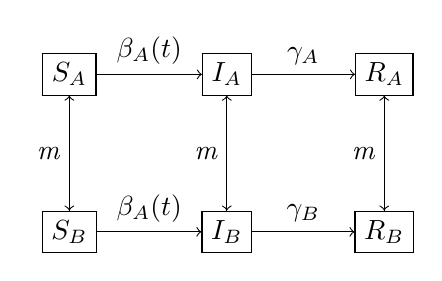
\begin{tikzpicture}
        % Nodes for patch 1
        \node[draw] (SA) at (0,0) {$S_A$};
        \node[draw] (IA) at (2,0) {$I_A$};
        \node[draw] (RA) at (4,0) {$R_A$};
        
        % Nodes for patch 2
        \node[draw] (SB) at (0,-2) {$S_B$};
        \node[draw] (IB) at (2,-2) {$I_B$};
        \node[draw] (RB) at (4,-2) {$R_B$};
        
        \draw[->] (SA) -- node[midway,above] {$\beta_A(t)$} (IA);
        \draw[->] (SB) -- node[midway,above] {$\beta_A(t)$} (IB);

        \draw[->] (IA) -- node[midway,above] {$\gamma_A$} (RA);
        \draw[->] (IB) -- node[midway,above] {$\gamma_B$} (RB);

        % Migration edges
        \draw[->] (SA) -- node[midway, left] {$\textit m$} (SB);
        \draw[->] (SB) -- (SA);
        \draw[->] (IA) -- node[midway, left] {$\textit m$}  (IB);
        \draw[->] (IB) -- (IA);
        \draw[->] (RA) -- node[midway, left] {$\textit m$}  (RB);
        \draw[->] (RB) -- (RA);

\end{tikzpicture}
\end{document}
